\documentclass[10pt, aspectratio=169]{beamer}
\AtBeginEnvironment{table}{\setlength\belowcaptionskip{0pt}}

\usepackage[utf8]{inputenc}
\usepackage{amsmath}
\usepackage{amsfonts}
\usepackage{amssymb}
\usepackage{graphicx}
\usepackage{ragged2e}  % `\justifying` text
\usepackage{booktabs}  % Tables
\usepackage{tabularx}
\usepackage{tikz}      % Diagrams
\usetikzlibrary{calc, shapes, backgrounds}
\usepackage{amsmath}
\usepackage{amssymb}
\usepackage{dsfont}
\usepackage{url}       % `\url
\usepackage{listings}  % Code listings
\usepackage[T1]{fontenc}
% \usepackage{caption}
% \usepackage[font=footnotesize]{caption}
% \captionsetup{skip=0pt,belowskip=0pt}
\usepackage{subcaption}
\usepackage[sort]{natbib}
\usepackage{adjustbox}
\usepackage{multicol}

% \setlength{\intextsep}{10pt plus 2pt minus 2pt}

\usepackage{theme/beamerthemehbrs}

\author[Jaswanth]{Jaswanth Bandlamudi \newline \newline \underline{Supervisors} \newline \vfill Prof. Dr. Paul G Pl\"{o}ger\\Prof. Dr. Nico Hochgeschwender \\ Prof. Dr. Matias Valdenegro Toro \\ M.Sc. Octavio Arriaga}
\title{Benchmarking Out-of-Distribution Detection in 2D Object Detection}
\subtitle{Thesis Defense}
\institute[HBRS]{Hochschule Bonn-Rhein-Sieg}
\date{\today}
% \subject{Test beamer}

\thirdpartylogo{images/DFKI.jpeg}


\begin{document}
\setlength{\parskip}{1em}
\renewcommand{\baselinestretch}{1.25}
{
\begin{frame}
\titlepage
\end{frame}
}

\setlength\abovecaptionskip{-5pt}
\section{Introduction}
\begin{frame}{Introduction}
\begin{itemize}
    \item Deep Neural Networks, current State-Of-The-Art (SOTA) performers in 
    \begin{itemize}
        \item Classification
        \item Object Detection
        \item Segmentation
    \end{itemize} 

    \item Trained with \textcolor{red}{\textit{closed world assumption}}, test data $\sim$ train data
    \item Deployed in open world $\implies$ Out-of-Distribution(OOD) examples
    \item Applications
        \begin{itemize}
            \item \textcolor{green}{Product recommendations}, recoverable
            \item \textcolor{orange}{Time series prediction}, partially reversible
            \item \textcolor{red}{Autonomous driving / Medical diagnosis}, irreversiable and catastrophic
        \end{itemize}
\end{itemize}
\end{frame}
\section{Problem Overview}
\begin{frame}{Out-of-Distribution (OOD) detection (1/3)}
    \begin{itemize}
        \item What is OOD data ?
        \begin{itemize}
            \item Data that is outside the semantic space formed by the images used for training
            \item Input with objects which are not used in training but have features closer to the object of
            interest.
        \end{itemize}
        
        \begin{figure}
            \centering
            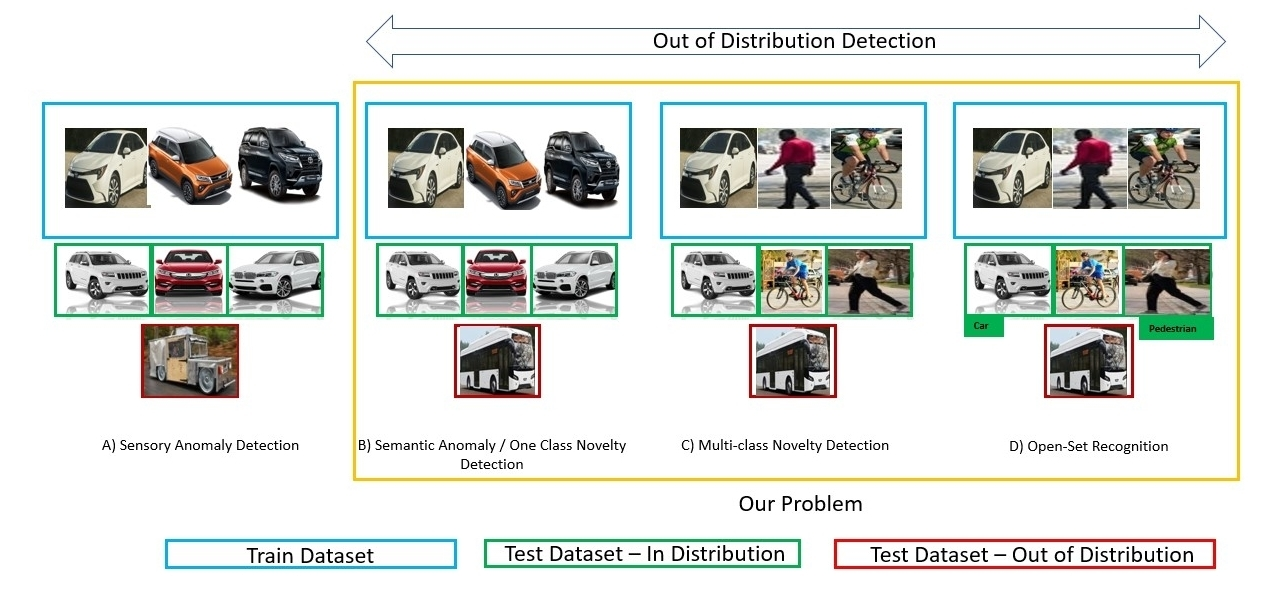
\includegraphics[scale=0.215]{images/OOD_vs_Non-OOD.jpg}
            \caption[\acrlong{ood} detection problem setting]{Class differentiation in generalized OOD detection framework}
            \label{fig:OOD_classes}
        \end{figure}
    \end{itemize}
\end{frame}

\begin{frame}{Out-of-Distribution (OOD) detection(2/3)}
    Different types of OOD data
    \begin{itemize}
        \item Data from a different domain
        \item Data with poor quality of features
        \item Data with inputs that are neither used nor prominent in the training data
    \end{itemize}
\end{frame}

\begin{frame}{Out-of-Distribution (OOD) detection(3/3)}
    Current Object Detection model performance on OOD data
    \begin{figure}[!htbp]
        \centering
      \subcaptionbox{\label{fig:1}}{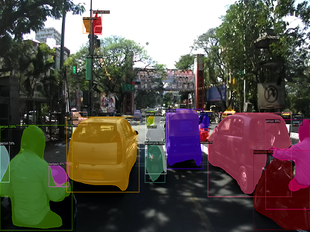
\includegraphics[scale=0.5]{images/False_Positive.png}}%\hspace{1em}
      \subcaptionbox{\label{fig:2}}{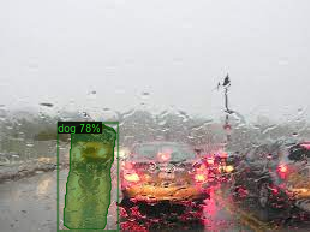
\includegraphics[scale=0.5]{images/False_Negative.png}}
      \caption[Sample False Positive and False Negative detections]{Examples of failures in object dedtection}
      \label{fig:3}
    \end{figure}
\end{frame}
\section{Solution}

\begin{frame}{OOD detector - Expectations}
    \begin{itemize}
        \item Produce a \textbf{\textit{Novelty Score (NS)}}. 
        \item NS can be a distance metric, a class-dependent probabilistic value, an entropy value, or a descriptive statistic value
        \item OOD detection can be posed as a binary classification problem.
    \end{itemize}
        
    
    
% \end{frame}

% \begin{frame}{Novelty Score - Behavior}
    
    % \begin{minipage}[t]{0.5\textwidth}
    %     $ X=
    %     \begin{cases}
    %         \text{ID}, & \text{if}\ NS \geq \delta \\
    %         \text{OOD}, & \text{otherwise} 
    %     \end{cases}
    %     $
    % \end{minipage} %%%
    % \begin{minipage}[t]{0.5\textwidth}
    %     \begin{figure}[H]
    %         \centering
    %         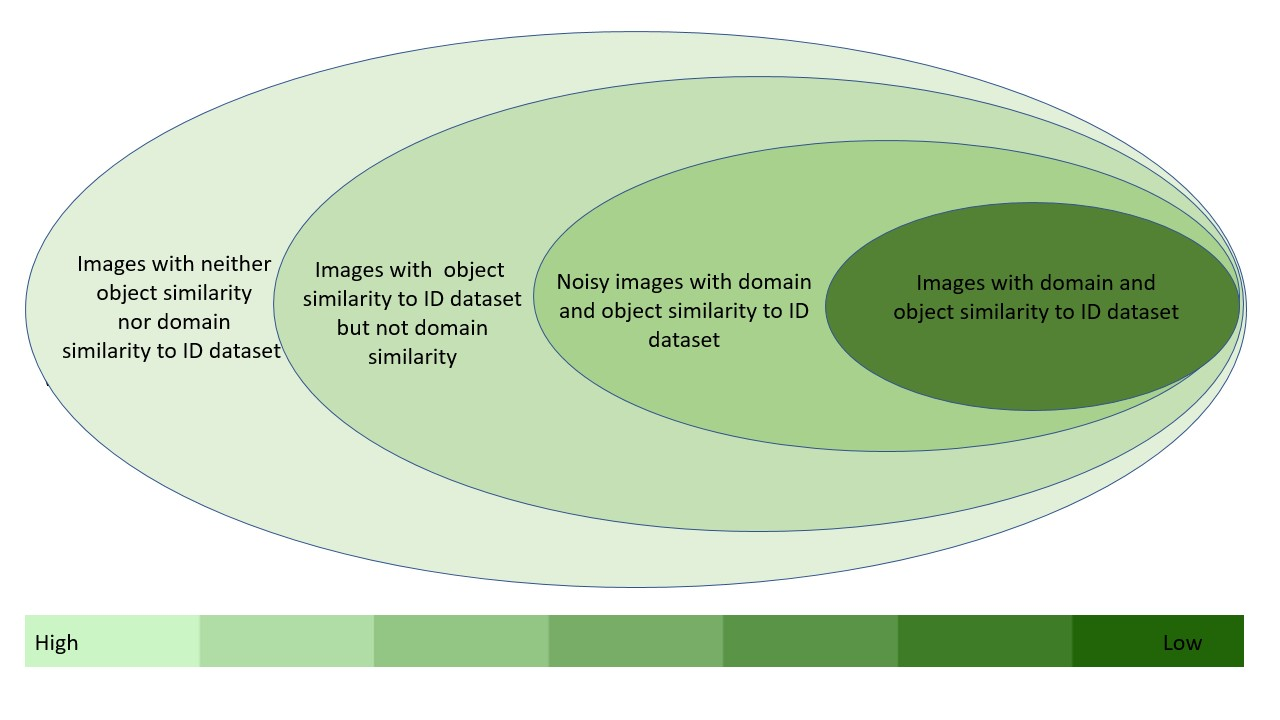
\includegraphics[scale=0.15]{images/Slide2.jpg}
    %         \caption[Novelty Score behavior]{Expected behavior of novelty score based on the nature of the OOD input}
    %         \label{fig:OD2_features}
    %     \end{figure}
    
    % \end{minipage}

    \begin{equation}
        \vcenter{\hbox{
            \begin{minipage}{5cm}
                \centering
                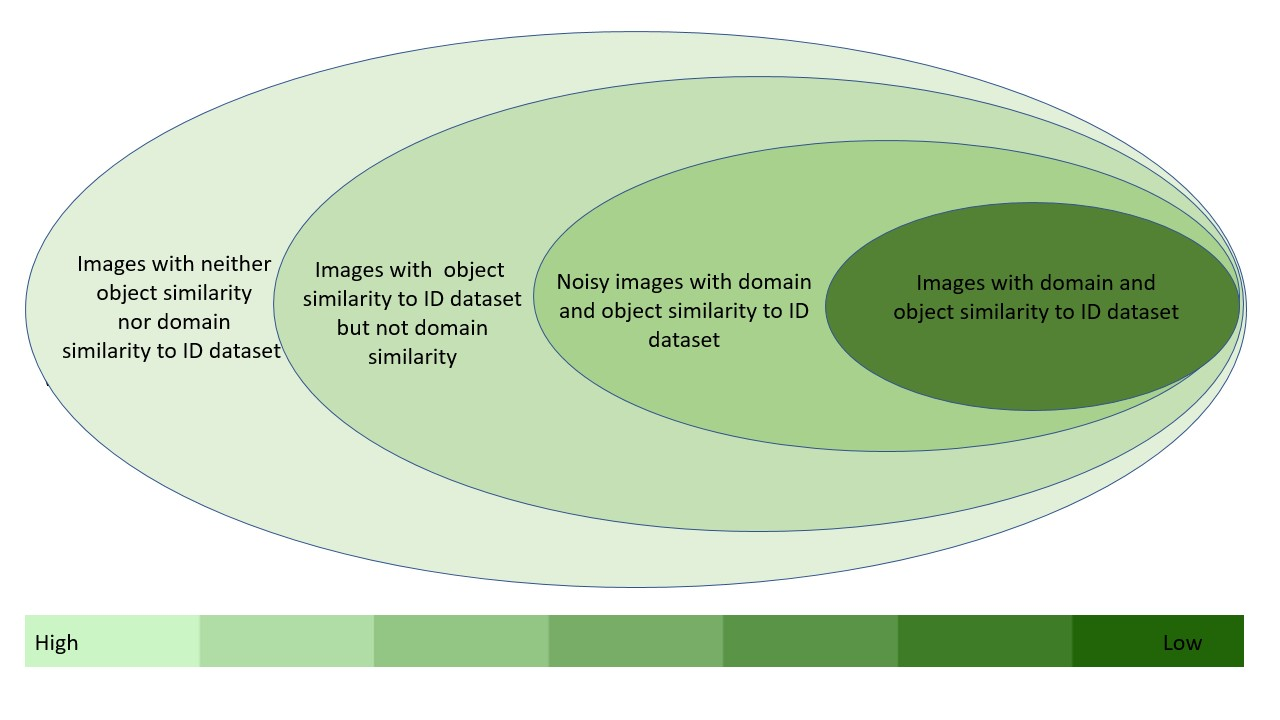
\includegraphics[scale=0.15]{images/Slide2.jpg}
                \captionof{figure}{Expected behavior of OOD detector.}
            \end{minipage}}}
        \qquad\qquad
        \begin{aligned}
            X=
                \begin{cases}
                    \text{ID}, & \text{if}\ NS \geq \delta \\
                    \text{OOD}, & \text{otherwise} 
                \end{cases}
        \end{aligned}
    \end{equation}

\end{frame}

\section{Previous works}
\begin{frame}{Previous works}
    \begin{table}[]
        \centering
        \caption{Previous works on OOD detection}
        \label{tab:my-table}
            \begin{tabular}{ll}
                \textbf{Method}             & \textbf{Works Proposed} \\ \hline
                Metric based methods        & \begin{tabular}[c]{@{}l@{}}\citet{Devries},  \citet{Oberdiek2018}, \\  \citet{Hendrycks2018} , \citet{Lee2018}\end{tabular} \\\hline
                Inconsistency based methods & \citet{liang2017enhancing} \\ \hline
                Generative methods          & \begin{tabular}[c]{@{}l@{}}\citet{Hendrycks2017},  \citet{Ren2019}, \\  \citet{VanDenOord2016}\end{tabular}    \\ \hline
                Uncertainty based methods   & \begin{tabular}[c]{@{}l@{}}\citet{Malinin2018},  \citet{Lakshminarayanan2017}, \\  \citet{VanAmersfoort2020} \\ \end{tabular}                       
            \end{tabular}
    \end{table}
    \begin{itemize}
        \item Works only for classification problem
        \item Not directly adaptable to object detection problem   
    \end{itemize}    
\end{frame}
\section{Methodology}
% \begin{frame}{Methodology}
%     In this work
%     \begin{itemize}
%         \item Proposed new benchmark dataset \textbf{Out of Distribution for Object Detection} ($OD^2$) dataset
%         \item Single-Shot Detector (SSD) is used to solve the object detection problem.
%         \item For OOD detection we decided to use
%         \begin{enumerate}
%             \item Max-Softmax score based OOD detection \citep{hendrycks17baseline}
%             \item ODIN \citep{liang2017enhancing}
%             \item Mahalanobis distance based OOD detection \citep{Lee2018}
%             \item Uncertainty based OOD detection \citep{Malinin2018, Lakshminarayanan2017}
%                 \begin{itemize}
%                     \item Bayesian Neural Network
%                     \item Sub-Ensemble
%                 \end{itemize} 
%         \end{enumerate}
%     \end{itemize}
% \end{frame}
\begin{frame}{$OD^2$ Dataset}
    \begin{table}[H]
        \centering
        \renewcommand{\arraystretch}{1.5}
        \caption{Table showing various type of images to address the OOD cases}
        \begin{adjustbox}{width=1\textwidth}
            \begin{tabular}{lllll}
            \hline
            \textbf{Purpose} & \textbf{Dataset Source} & \textbf{Classes} & \textbf{Novelty Score Behavior} & \textbf{Task} \\ \hline
            In-Distribution & BDD100K \citep{bdd100k} & \begin{tabular}[c]{@{}l@{}}Pedestrian, Rider, Car, Truck, Bus, \\ Motorcycle, Bicycle, Traffic sign\end{tabular} & Low Novelty score  & \begin{tabular}[c]{@{}l@{}}Object detector \\ performance \end{tabular} \\ \hline
            \begin{tabular}[c]{@{}l@{}}Low light and \\ bad image quality\end{tabular} & \begin{tabular}[c]{@{}l@{}}BDD100K (non-clear weather) \\ and Climate-GAN \citep{climategan} \\generated Smog images\end{tabular} & \begin{tabular}[c]{@{}l@{}}Pedestrian, Rider, Car, Truck, Bus, \\ Motorcycle, Bicycle, Traffic sign\end{tabular} & Medium Novelty Score   & Detector Robustness\\ \hline
            \begin{tabular}[c]{@{}l@{}}Classes with \\ semantic-variance\end{tabular}  & IDD \citep{Varma2019IDDAD} & Trucks, Motorcycles, Traffic Sign & High Novelty Score     & OOD detection\\ \hline
            Novel Classes  & IDD & Auto-Rickshaws  & High Novelty Score     & \begin{tabular}[c]{@{}l@{}}Multi class \\ novelty detection \end{tabular} \\ \hline
            \begin{tabular}[c]{@{}l@{}}Out-of-Domain \\ images\end{tabular} & \begin{tabular}[c]{@{}l@{}}Climate-GAN generated \\ Flood and Fire images\end{tabular} & \begin{tabular}[c]{@{}l@{}}Pedestrian, Rider, Car, Truck, Bus, \\ Motorcycle, Bicycle, Traffic sign\end{tabular} & High Novelty Score & \begin{tabular}[c]{@{}l@{}}Out-Of-Domain \\ detection \end{tabular}\\ \hline
            \end{tabular}
        \end{adjustbox}
        \label{dataset_summary}
    \end{table}
\end{frame}

\begin{frame}[allowframebreaks]{Single Shot multi-box Detector (SSD) model}
    \begin{figure}[!ht]
        \centering
        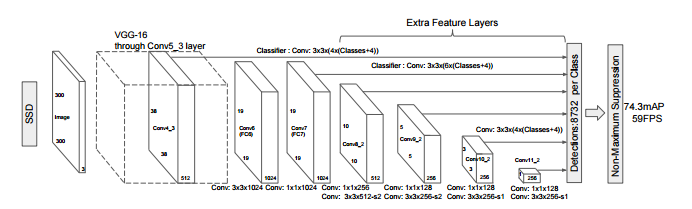
\includegraphics[scale=0.45]{images/SSD.png}
        \caption[SSD framework]{SSD framework proposed by \citet[p. 24]{Liu2016SSDSS}.}
        \label{fig:Fr-RCNN}
    \end{figure}
    \smallskip
    \begin{multicols}{2}
        \begin{itemize}
            \item Single network for detection and classification
            \item No Fully-Connected layers
            \item Low input resolution
        \end{itemize}
    \end{multicols}
% \end{frame}

% \begin{frame}{Single Shot multi-box Detector (SSD) model}
    \begin{multicols}{2} % two columns
        \begin{itemize}
            \item Default boxes
            \item Matching strategy is used,
                \begin{itemize}
                    \item $ IoU_{default box}^{ground truth}$ > 0.5
                    \item overlapped objects and simple learning 
                \end{itemize}
                
            \item Processing of features from multiple layers
                \begin{itemize}
                    \item Deep feature maps
                    \item Shallow feature maps
                \end{itemize}
        \end{itemize}

        \begin{itemize}
            \item Loss
            $$L(x, c, l, g)=\frac{1}{N}\left(L_{\text {conf }}(x, c)+\alpha L_{\text {loc }}(x, l, g)\right)$$
            \begin{itemize}
                \item $L_{conf}$ is Softmax Loss
                \item $L_{loc}$ is Smooth $L_{1}$ Loss 
            \end{itemize}
            \item Filter boxes with low confidence and NMS with 0.45 IOU
            \item Top 200 detections are considered
            
        \end{itemize}
    \end{multicols}
\end{frame}

\begin{frame}[allowframebreaks]{OOD methods}
    \begin{itemize}
        \item Max-Softmax
        
        Maximum value of softmax scores are used as novelty score
        \begin{equation}
            \setlength{\jot}{10pt}
                s\left(\mathbf{x}^{*}\right)=\max _{c} P\left(y_{c} \mid \mathbf{x}^{*} ; \mathcal{D}\right)
                \label{softmax_score}
        \end{equation}

        \item ODIN
        
        \begin{equation}
            \tilde{\boldsymbol{x}}=\boldsymbol{x}-\operatorname{esign}\left(-\nabla_{\boldsymbol{x}} \log S_{\hat{y}}(\boldsymbol{x} ; T)\right)
            \label{perturbation}
        \end{equation}

        \begin{equation}
            S_{i}(\boldsymbol{x} ; T)=\frac{\exp \left(f_{i}(\boldsymbol{x}) / T\right)}{\sum_{j=1}^{N} \exp \left(f_{j}(\boldsymbol{x}) / T\right)}
            \label{ODIN_Softmaxscore}
        \end{equation}

        \begin{itemize}
            \item $\epsilon$ is the perturbation magnitude
            \item $T$ is the Temperature
        \end{itemize}
        
        \newpage
        
        \item Mahalanobis distance based OOD detection
        
        assuming intermediate layer features follow class-conditional Gaussian distributions with tied covariances

        % \begin{equation}
        %     M(x)=\max _{c}-\left(f(x)-\hat{\mu}_{c}\right)^{T} \hat{\Sigma}^{-1}\left(f(x)-\hat{\mu}_{c}\right), where. \\
        %     & \hat{\mu}_{c}=\frac{1}{N_{c}} \sum_{i: y_{c}=c} f\left(x_{i}\right) \\
        %     & \hat{\Sigma}=\frac{1}{N} \sum_{c} \sum_{i: y_{c}=c}\left(f\left(x_{i}\right)-\hat{\mu}_{c}\right)\left(f\left(x_{i}\right)-\hat{\mu}_{c}\right)^{T} \\
        % \end{equation}

        \begin{equation}
            M(x)=\max _{c}-\left(f(x)-\hat{\mu}_{c}\right)^{T} \hat{\Sigma}^{-1}\left(f(x)-\hat{\mu}_{c}\right)
        \end{equation}

        $$\hat{\mu}_{c}=\frac{1}{N_{c}} \sum_{i: y_{c}=c} f\left(x_{i}\right)$$
            
        $$\hat{\Sigma}=\frac{1}{N} \sum_{c} \sum_{i: y_{c}=c}\left(f\left(x_{i}\right)-\hat{\mu}_{c}\right)\left(f\left(x_{i}\right)-\hat{\mu}_{c}\right)^{T} $$ \newline \newline \newline
        
        \item Uncertainty based OOD detection
        \begin{itemize}
            \item Bayesian Neural Network
            \begin{columns}
                \column{0.38\linewidth}
                   \centering
                   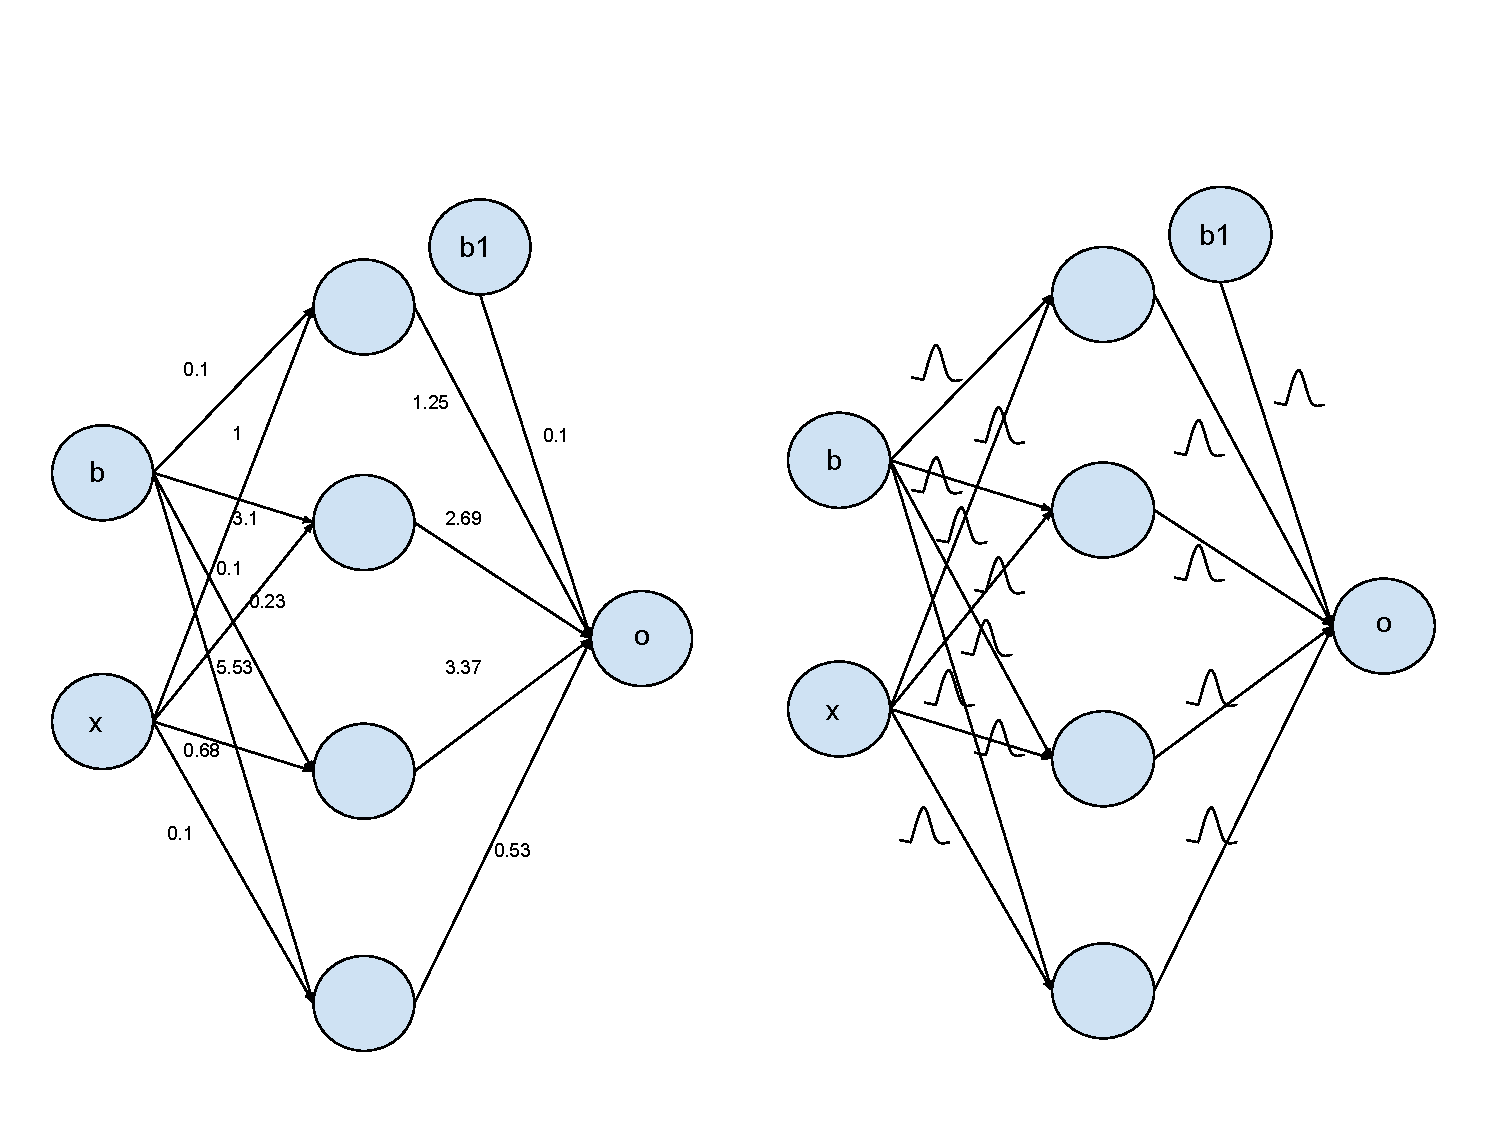
\includegraphics[scale=0.275]{images/BNN.pdf}
                 \column{0.38\linewidth}
                    \begin{itemize}
                        \item Bayesian Flipout layers \citep{Wen2018}
                        \item Reparameterization trick for training \citep{Kingma2015}
                        \item Prior $P(w)$ $\sim$ $N(0, 1)$
                        \item multiple forward passes for uncertainty quantification
                    \end{itemize}
            \end{columns} \newpage
        
            \item Sub-Ensemble Network 
            \begin{columns}
                \column{0.38\linewidth}
                   \centering
                   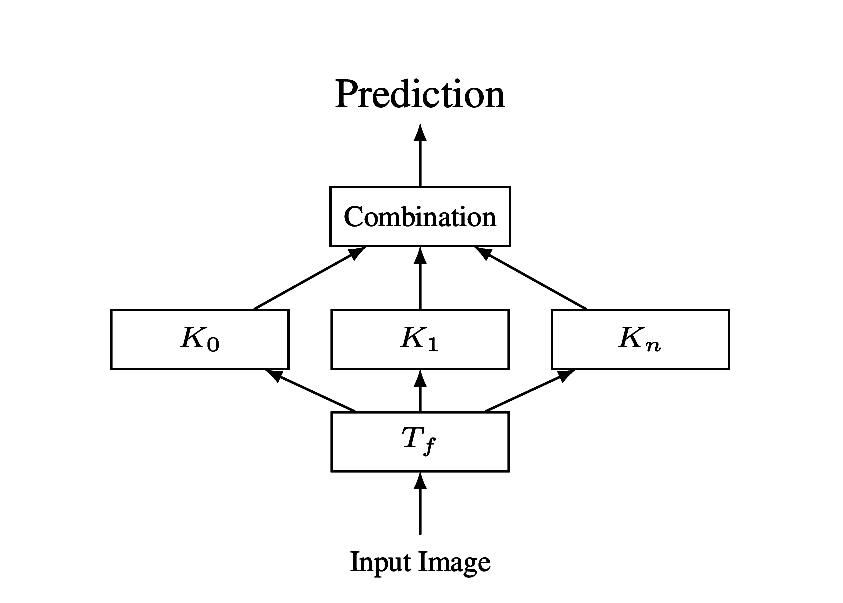
\includegraphics[scale=0.275]{images/subensembles.png}
                 \column{0.38\linewidth}
                    \begin{itemize}
                        \item Model is divided into Trunk and Task layers
                        \item Trunk layers has best performing weights restored and cannot be trained
                        \item Task layers are randomly initialized and re-trained
                        \item Random initialization of layers creates ensemble model. 
                    \end{itemize}
            \end{columns} \newpage
            \item Novelty Score \newline
            
            Entropy
            \begin{equation}
                \label{Entropy}
                \begin{array}{l}
                    \text{Entropy} =-\sum_{i=1}^{C} P\left(c_i \mid \mathbf{x}^{*} ; \mathcal{D}\right) \ln P\left(c_i \mid \mathbf{x}^{*} ; \mathcal{D}\right) 
                \end{array}
            \end{equation} \newline

            Box deviation is the square root of the trace of the covariance matrix $C(x^{*})$.
            \begin{equation}
                C\left(\mathbf{x}^{*}\right)=\frac{1}{N} \sum_{i=1}^{N} \hat{\mathbf{v}}_{\mathbf{x}^{*}}^{i} \hat{\mathbf{v}}_{\mathbf{x}^{*}}^{i^{T}}-\mathbf{I}_{\mathbf{x}^{*}} \mathbf{I}_{\mathbf{x}^{*}}^{T}
            \end{equation}

        \end{itemize}
    \end{itemize}
\end{frame}

\section{Results}
\begin{frame}{SSD Object Detection Results}

    \begin{figure}%
        \centering
        % \subfloat[]{{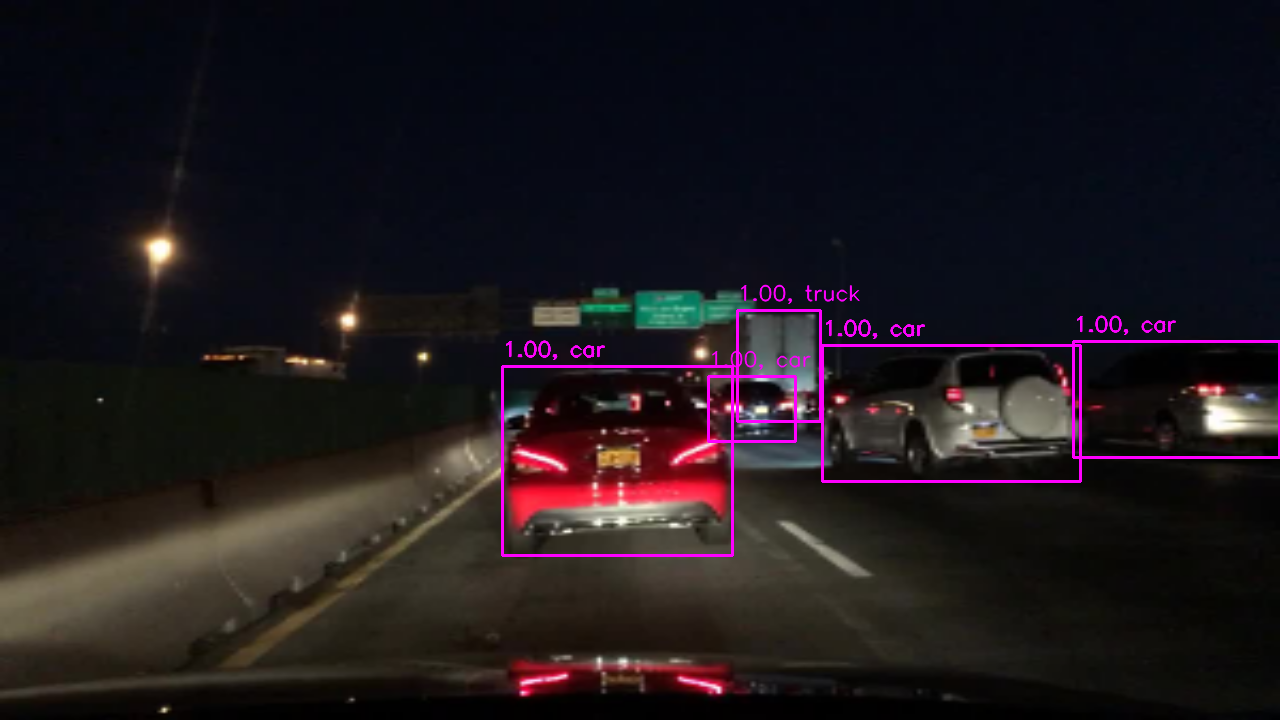
\includegraphics[height=3.5cm, width=6cm]{images/9.png} }}%
        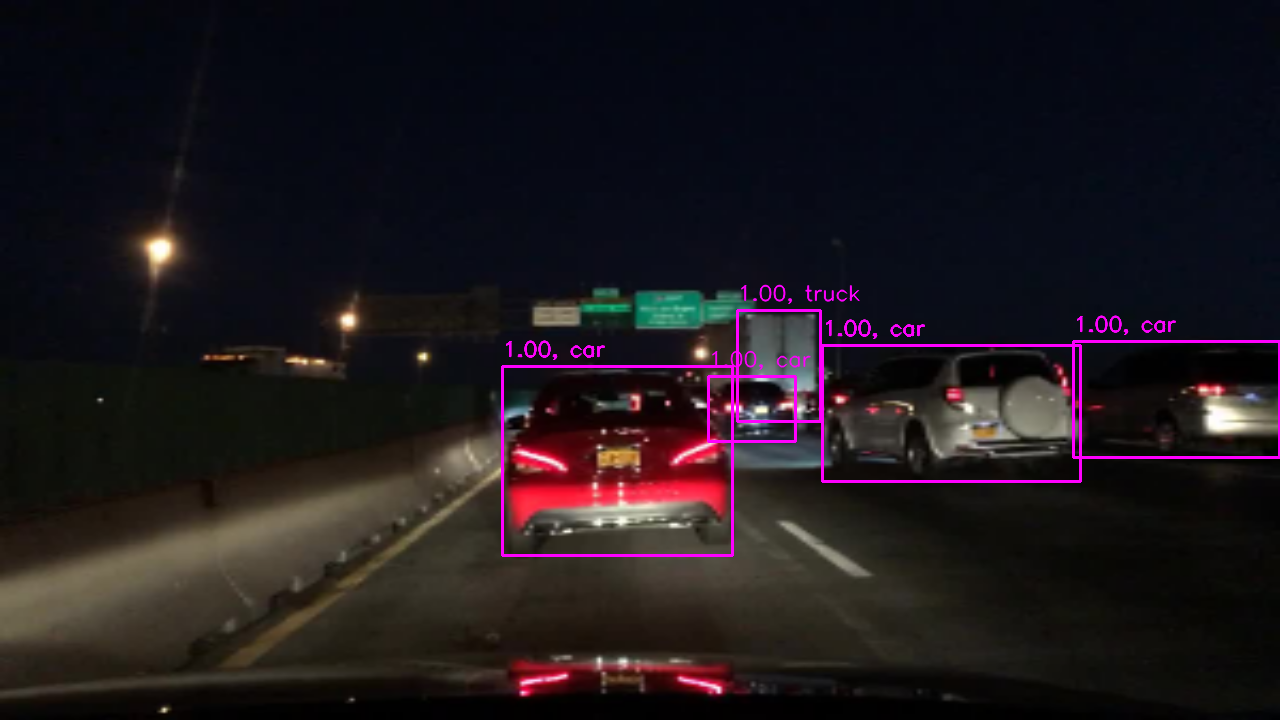
\includegraphics[width=6cm, height=3.5cm]{images/9.png}
        % \qquad
        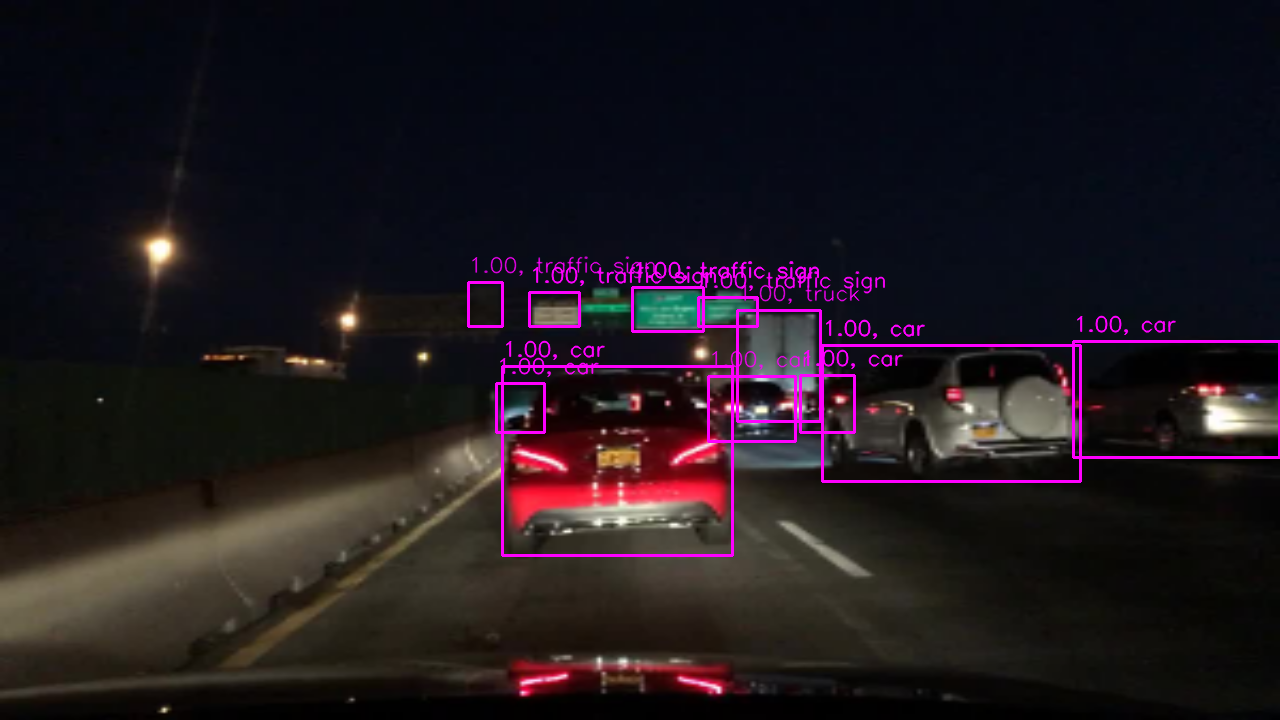
\includegraphics[width=6cm, height=3.5cm]{images/tuned_9.png}
        % \subfloat[]{{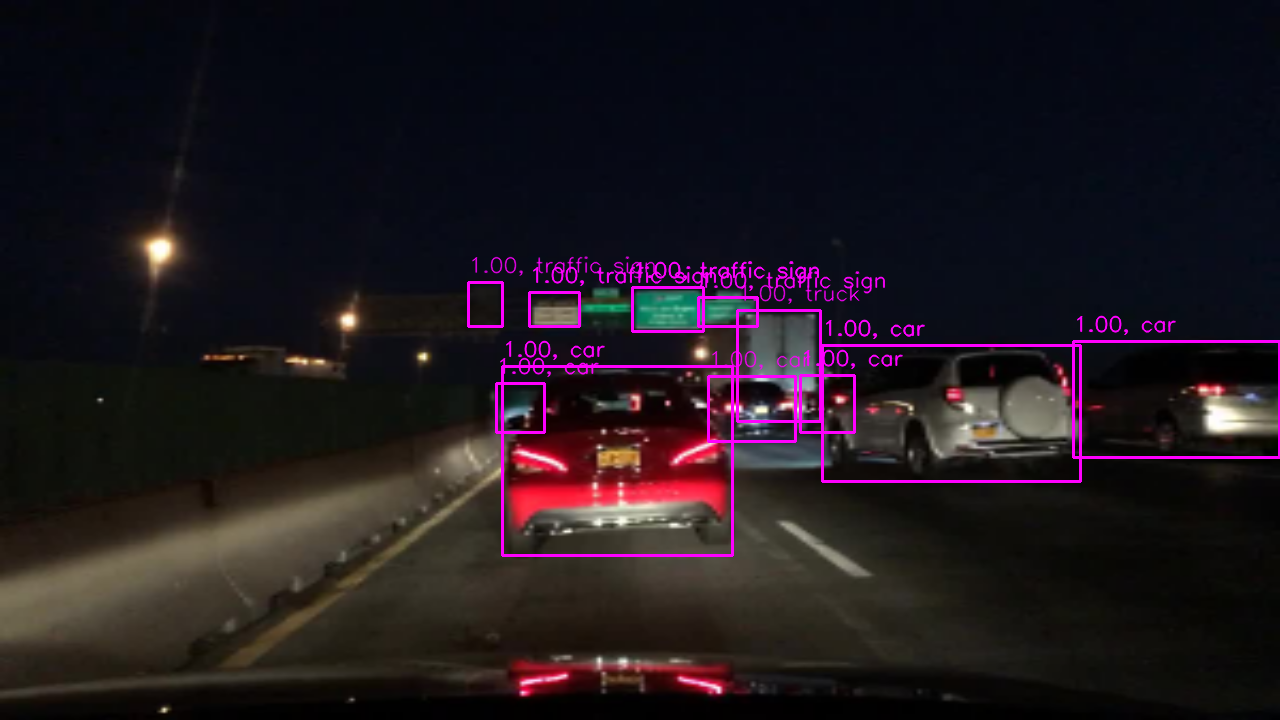
\includegraphics[height=3.5cm, width=6cm]{images/tuned_9.png} }}%
        \caption{Matched prior boxes and ground truth boxes}%
        \label{fig:example}%
    \end{figure}

    % \begin{figure}[H]
    %     \centering
    %     \begin{minipage}{.5\textwidth}
    %       \centering
    %       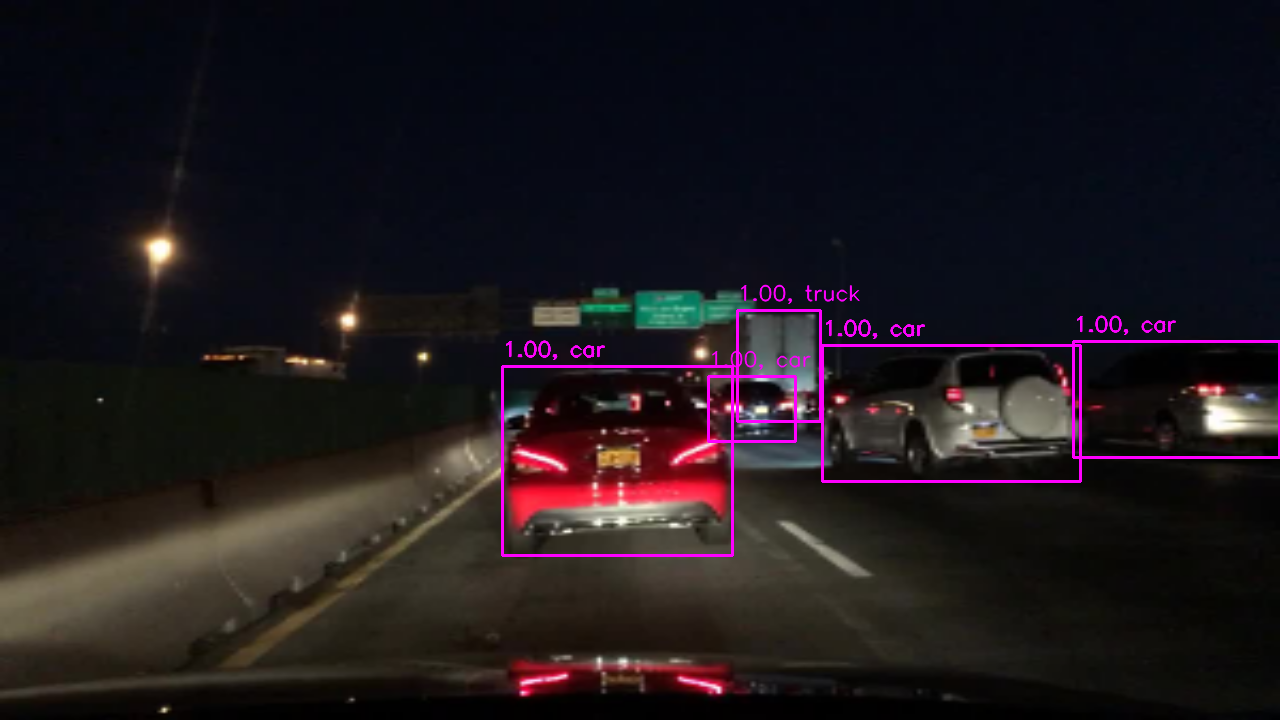
\includegraphics[width=6cm, height=3.5cm]{images/9.png}
    %     \end{minipage}%
    %     \begin{minipage}{.5\textwidth}
    %       \centering
    %       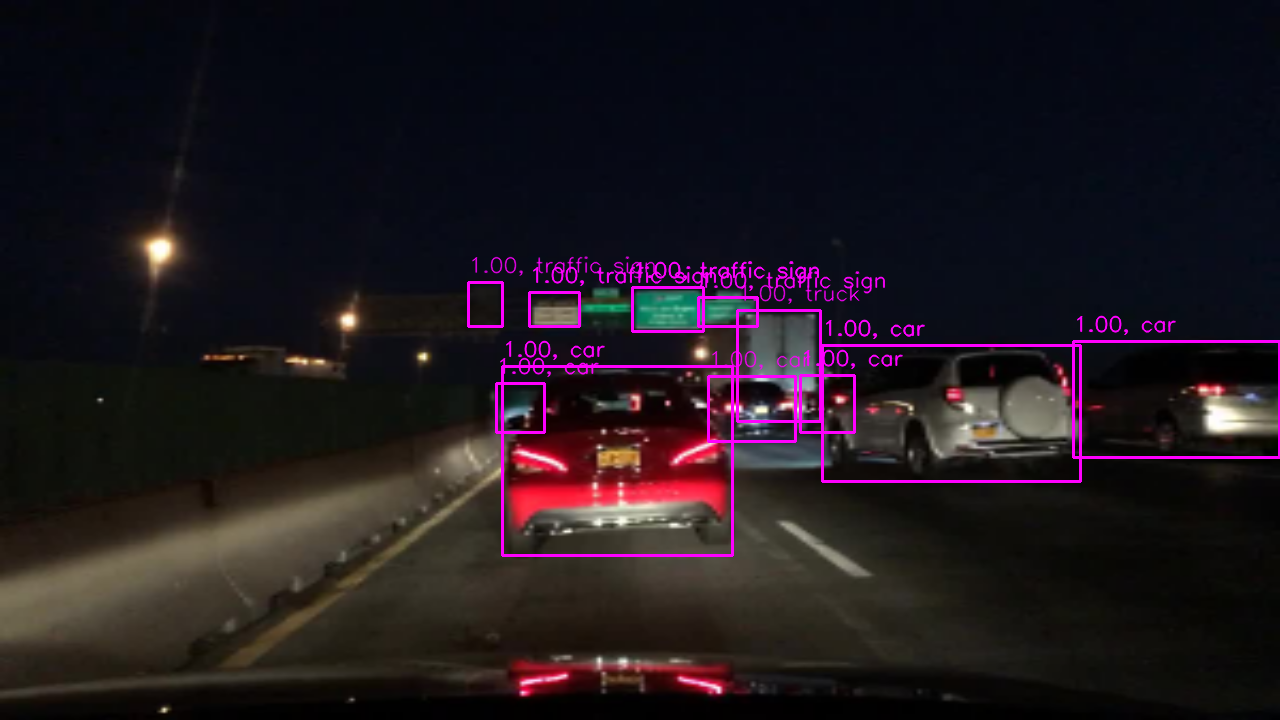
\includegraphics[width=6cm, height=3.5cm]{images/tuned_9.png}
    %     \end{minipage}
    %     \caption{Matched prior boxes and ground truth boxes}
    % \end{figure}

    \begin{table}[]
        % \renewcommand{\arraystretch}{1.5}
        \caption{Average Precision values using SSD300 model with and without tuned prior boxes}
        \resizebox{\textwidth}{!}{
    \scriptsize \begin{tabular}{cllllllllll}
    
                                  &                         & \multicolumn{9}{c}{\textbf{Agents}}  \\ \hline
                                  & \multicolumn{1}{l}{\textbf{Models}}         & \multicolumn{1}{l}{\textbf{Pedestrian}} & \multicolumn{1}{l}{\textbf{Rider}} & \multicolumn{1}{l}{\textbf{Car}} & \multicolumn{1}{l}{\textbf{Truck}} & \multicolumn{1}{l}{\textbf{Bus}} & \multicolumn{1}{l}{\textbf{Motorcycle}} & \multicolumn{1}{l}{\textbf{Bicycle}} &\multicolumn{1}{l}{\textbf{Traffic Sign}} & \textbf{mean} \\ \hline
     & \multicolumn{1}{l}{\textbf{SSD300}}         & \multicolumn{1}{l}{0.006}               & \multicolumn{1}{l}{0.004}          & \multicolumn{1}{l}{0.095}        & \multicolumn{1}{l}{0.083}          & \multicolumn{1}{l}{0.15}         & \multicolumn{1}{l}{0.045}               & \multicolumn{1}{l}{0.092}            & \multicolumn{1}{l}{0.001}       &     0.059     \\ \cline{1-11} 
                                  & \multicolumn{1}{l}{\textbf{SSD300 - Tuned}} & \multicolumn{1}{l}{0.165}               & \multicolumn{1}{l}{0.135}          & \multicolumn{1}{l}{0.479}        & \multicolumn{1}{l}{0.389}          & \multicolumn{1}{l}{0.389}        & \multicolumn{1}{l}{0.163}               & \multicolumn{1}{l}{0.213}            & \multicolumn{1}{l}{0.186}    &     0.265        \\ \hline
    \end{tabular}
            }
            \label{map_basic}
        \end{table}


\end{frame}


\begin{frame}[allowframebreaks]
    \frametitle{References}
    \bibliographystyle{unsrtnat}
    % \bibliography{bibliography.bib}
    {\small
\bibliography{bibliography.bib}}
\end{frame}
\end{document}
